In this section, we first describe the data sets used in our
experimental study. After that, we present the experiments to evaluate
our approach at different levels: our local classifier only, local
classifier pluses going beyond Wikipedia, and pluses constrant-based
inference model with related concepts from gold data and YAGO
ontology. We then compare our results with other related work and
perform several experimental analyses.

\subsection{Datasets}
\label{sec:dataset}

Our approach to identifying relational knowledge is evaluated by using
a dataset of 40 semantic classes of almost 11,000 instances, which was
used in \cite{citeulike:1587018}.  This dataset was manually
constructed\footnote{Private communication with Marius Pasca, 2009.}
and was used to evaluate many information extraction tasks
\cite{citeulike:1587018,pacsca-vandurme:2008:ACLMain}.  Each semantic
class is an incomplete set of representative instances and has about
272 instances in average. The smallest class is {\em search engine}
with 25 instances, and the largest class is {\em actor} with 1500
instances. Table \ref{table:class-instance} shows a snippet of the
dataset. Interestingly, we have both types of closed word semantic
class (e.g. {\em chemical element}, {\em country}) and open word
semantic class (e.g. {\em basic food}, {\em hurricane}). Moreover,
there are classes with proper nouns (e.g. {\em actor} with {\em Mel
  Gibson}, {\em Sharon Stone}) and classes with common nouns
(e.g. {\em basic food} with {\em rice}, {\em milk}, {\em eggs}). With this
data set, we can evaluate the ability of our system in dealing with not only
name entity concept, but also common noun concepts.

\begin{table}[h]
\small
  \centering
  \begin{tabular}{|r|l|}
    \hline
    \textbf{Semantic class (Size)} & \textbf{Examples of Instances} \\
    \hline
    \hline
    basic food (155) & rice, milk, eggs, beans, fish \\
    \hline
    chemical element (118) & lead, copper, aluminum, calcium \\
    \hline
    city (589) & San Francisco, Dubai, Chicago \\
    \hline
    disease (209) & arthritis, hypertension, influenza \\
    \hline
    actor (1500) & Kate Hudson, Mel Gibson \\
    \hline
  \end{tabular}
  \caption{A snippet of 40 semantic classes with instances. 
    The class names in the original dataset ({\em basicfood}, 
    {\em chemicalelem}) were presented in a meaningful form
    as shown in the left column.}
  \label{table:class-instance}
\end{table}

In the original dataset, the semantic class names are not often
written in a meaningful form, such as {\em chemicalelem}, {\em
  proglanguage}, and {\em worldwarbattle}. These names are not valid
concepts. In our experiments, each semantic class name in the original
dataset is expanded to meaningful forms. For example, {\em
  terroristgroup} is expanded to {{\em terrorist group}, {\em
    terrorrist}, {\em torrorism}}. We use these expansions for all
systems in the experiments.

% We refer to these expansions as {\em class expansion}.

An example in our learning problem is a pair of two concepts ($X$,
$Y$) such as ({\em city}, {\em Dubai}), ({\em lead}, {\em
  aluminum}). Note that in this paper, we refer to both the name of
the semantic classes and their instances as concepts, such as {\em
  city} and {\em Dubai}. We pair the semantic classes and instances in
the original data set to create training and testing examples. The
examples cover all types of relational knowledge of interest: $X
\leftarrow Y$, $X \rightarrow Y$, $X \leftrightarrow Y$, and $X
\nleftrightarrow Y$. Specifically, examples are created with the
following guidelines.

\begin{itemize}
\item $X \leftarrow Y$ examples: For each semantic class, we pair the
  name of the class with its instances. These examples have the
  genearl form ({\em semantic class X}, {\em child of X}).
\item $X \rightarrow Y$ examples: These examples have the general form
  ({\em concept X}, {\em semantic class of X}).
\item $X \leftrightarrow Y$ examples: The general form of these
  examples is ({\em concept X}, {\em concept Y}), where $X$ and $Y$
  are two instances of a semantic class, and $X \ne Y$.
\item $X \nleftrightarrow Y$ examples: To make examples with two
  concepts having no relation, we pair either a semantic class name
  and an instance of another semantic class (and vice versa), or an
  instance in a semantic class and another instance in other classes.
\end{itemize}

Tab. \ref{table:examples} shows some examples created from the
original data set.

\begin{table}[h]
  \centering
  \begin{tabular}{|r|l|l|}
    \hline
    Relation          & Concept $X$ & Concept $Y$    \\
    \hline
    \hline
    $X \leftarrow Y$        & actor             & Mel Gibson           \\
    & food              & rice                 \\
    % & wine              & Champagne            \\
    \hline                               
    $X \rightarrow Y$       & Makalu            & mountain             \\
    & Monopoly          & game                 \\
    % & krooni            & currency             \\
    \hline                               
    $X \leftrightarrow Y$   & Paris             & London               \\
    & copper            & oxygen                \\
    % & Nile              & Volga                 \\
    \hline                               
    $X \nleftrightarrow Y$ & Roja              & C++                  \\
    & egg               & Vega                  \\
    % & HotBot            & autism                \\
    \hline
  \end{tabular}
  \caption{Some examples in our data set.}
  \label{table:examples}
\end{table}

We randomly create $20,000$ examples following the guidelines
above. From these examples, we use $8,000$ examples for the training
set, and $12,000$ examples for the test set. We refer to the
12,000-example test set as the {\em TestAll} test set.

From the training set, we discard examples with one or both concepts
not in Wikipedia ({\em non-Wikipedia examples}).  By using our concept
disambiguation algorithm (see Fig. \ref{fig:entity-disamb}), we can
discover {\em non-Wikipedia} examples by seeing if the algorithm
retrieves no relevant articles for either one or both concepts in the
examples. This results in a training set of $6,959$ examples.  It is
important to note that, we do not discard {\em non-Wikipedia} examples
in the {\em TestAll} test set. Table \ref{tab:detail-dataset} shows
the statistics of the training and testing data with the number of
examples in each relation class.

\begin{table}[h]
  \small
  \begin{center}
    \begin{tabular}{|l||c|c|c|c|c|}
      \hline
      Data & $X \leftarrow Y$ & $X \rightarrow Y$  & $X \leftrightarrow Y$  & $X \nleftrightarrow Y$ & Total \\
      \hline
      \hline
      {\em Training}  & 1,739 & 1,754 & 1,664 & 1,802 & 6,959\\
      % {\em TestWiki} & 2,684 & 2,654 & 2,483 & 2,635 & 10,456 \\
      {\em TestAll} & 3,045 & 3,025 & 2,965 & 2,965 & 12,000 \\
      \hline
    \end{tabular}
    \caption{Details of the training and test sets with the number of
      examples in each relation class. The {\em Training} set
      contains only examples in Wikipedia. {\em TestAll} includes {\em
        non-Wikipedia} examples.}
    \label{tab:detail-dataset}
  \end{center}
\end{table}

To evaluate our system, we use a snapshot of Wikipedia from July,
2008. We first clean up articles in Wikipedia and remove articles that
are not of interest. The removed articles include articles without a
category, except the redirect pages, or articles with useless
categories such as {\em Protected redirects}. We also remove
administrative articles including {\em Wikipedia} pages, {\em
  Template} pages, {\em Image} pages, and {\em Portal}
pages. Furthermore, we do not use articles without titles. After the
pre-processing step, we have 5,503,763 articles left. We index the
articles using the Apache Lucene Information Retrieval
library\footnote{http://lucene.apache.org, version 2.3.2}. Lucene is a
high-performance text search library written in Java that is a
widely used off-the-shelf IR system.

\subsection{Experimental Results}
\label{sec:exp-results}

\begin{table*}[t]
  \begin{center}
    \begin{tabular}{|c||c|c|c|c||c|c|}
      \hline
      {\em K}  &  {\em Local Classifier}  &  {\em +BeyondWiki}  &  \multicolumn{2}{|c||}{{\em +Inference (YAGO)}}  &  \multicolumn{2}{|c|}{{\em +Inference (Gold)}} \\ \cline{4-7}
      &          Accuracy  &            Accuracy  &            Accuracy  &  Error Reduction  &  Accuracy            &  Error Reduction  \\
      \hline
      \hline
      0  &             37.69  &               37.99  &               37.99  &              -    &  37.99               &           -       \\
      1  &             79.37  &               80.62  &               82.13  &           13.38   &  84.57               &         25.21     \\
      2  &             81.89  &               83.58  &               84.79  &           16.01   &  86.52               &         25.57     \\
      3  &             81.38  &               83.14  &               85.07  &           19.82   &  85.44               &         21.80     \\
      4  &              80.3  &                82.0  &               84.08  &           19.19   &  84.42               &         20.91     \\
      \hline
    \end{tabular}
    \caption{Performances in accuracy of our system, evaluated on {\em
        TestAll} test set. $K$ is the number of levels one goes up on
      the Wikipedia category system to extract features for input
      concepts. With $K=0$, no constraints are mined, the inference
      model is not used. '-' means the error reduction is too small.}
    \label{table:all-performances}
  \end{center}
\end{table*}

We evaluate our system at three different levels. The
first level evaluates our local relation classifier described in
Sec. \ref{sec:super-approach}. We refer to the first level as {\em
  Local Classifier}. In the second level, we apply our method
presented in Sec. \ref{sec:impr-syst-cover} to find replacements for
concepts that are not in Wikipedia. The results for this level are
presented under the name {\em +BeyondWiki}. For the third
level of evaluation, we use the approach described in
Sec. \ref{sec:constraints} to extract related concepts for input
examples from YAGO ontology to evaluate our constraint-based inference
model. We use the name {\em +Inference (YAGO)} to refer to the third
level experiment. Note that, {\em +Inference (YAGO)} is evaluated on
top of the results of {\em Local Classifier} and {\em +BeyondWiki}.
{\em +Inference (YAGO)} and shows our final results on the identification
problem of relational knowledge.

We also report the performance of our system in the third level of
evaluation using the related concepts added manually.  This
experiment, as mentioned in Sec.  \ref{sec:rel-con-ext}, shows the
correctness of our inference model.  To have gold related concepts, we
take advantage of our original data set described in
Sec. \ref{sec:dataset}. The original data set provides us ancestor and
sibling concepts for basic concepts such as {\em Chicago}, {\em
  hypertension}, etc., and children for generic concepts such as {\em
  chemical element}, {\em actor}, etc. We refer to this experiment as
{\em +Inference (Gold)} which is also evaluated on top of {\em Local
  Classifier} and {\em +BeyondWiki}. Furthermore, in this experiment,
for each input concept, we use 1 ancestor, 5 siblings, and 5 children
as its related concepts (i.e. 22 related concepts for an example) for
both {\em +Inference (YAGO)} and {\em +Inference (Gold)}.

In our system, we vary the value of $K$ as the number of levels that
one goes up on the Wikipedia category system to extract features (see
Sec. \ref{sec:super-approach}) for input concept pairs. In our
experiments, $K$ is set from $0$ to $4$.  We train our classifier on
the {\em Train} training set and evaluate on the {\em TestAll} test
set described in table \ref{tab:detail-dataset}. We evaluate
performance of the systems by calculating the accuracy of
identification of relations between concepts in pairs. Accuracy is
calculated by the percentage of the number of correct predictions over
the total number of examples used in testing. Table
\ref{table:all-performances} summarizes the performance of our system
at different levels of evaluation.

First of all, from Tab. \ref{table:all-performances}, we see that
without using the Wikipedia category system ($K=0$), we get very poor
performance. The situation changes significantly when the Wikipedia
category system is used. The best performance of the local relation
classifier is $81.89\%$ in accuracy. By using our approach to find
replacements for {\em non-Wikipedia} concepts (going beyond
Wikipedia), we get remarkable improvement with $83.58\%$ of accuracy
as the best performance. However, with $K=0$, the performance almost
remians the same. One of the reasons for this phenomenon is that although
{\em +BeyondWik} works well, we cannot expect to get good result with
a poor local classifier at $K=0$.

Significant improvement of the system's performance compared to {\em
  Local Classifier} is achieved when we use our constraint-base
inference model to predict concept relations. Except when $K=0$, all
other values of $K$ gain significant error reduction. The best
performance of our system is $85.07\%$ with $K=3$ when applying our
inference model on top of {\em Local Classifier} {\em +BeyondWiki},
gaining $19.82\%$ error reduction. All inference processes in this
experiment use $22$ related concepts for each input concept pair. With
$K=0$, the {\em forward constraint selection} algorithm returns no
constraint, therefore, the inference process does not help improving
the performance of the system.

On the other hand, the performance of {\em +Inference (Gold)} shows
that our constraint-based inference model using relational constraints
is correct and effective. The system using {\em +Inference (Gold)}
achieves the best performance -- $86.52\%$ accuracy, gaining $25.57\%$
error reduction. However, in real-world problems, the gold related
concepts are not available. Therefore, we propose using the YAGO
ontology to extract related concepts for the inference process to make
predictions for real-world input concept pairs. Importantly, the results
of the {\em +Inference (Gold)} experiment show that the more relevant
the related concepts are, the better performance our system achieves.

Table \ref{table:pre-examples} shows some output examples of our
system from the best setting ({\em Local Classifier} {\em +BeyondWiki}
\linebreak {\em +Inference(YAGO)}).  Example \#1 shows the case where
all levels of prediction are correct. In \#2, the local relation classifier
makes incorrect predictions, but then is corrected by {\em +BeyondWiki}
because {\em +BeyondWiki} finds a good replacement for non-Wikipedia
concept {\em bartlomiej strobel}. In examples \#3 and \#4, both {\em
  Local Classifier} and {\em +BeyondWiki} make incorrect predictions, but
{\em +Inference (YAGO)} remedies these. Example \#5 shows an
interesting case where the local classifier itself, by some chance,
makes correct prediction, but {\em +BeyondWiki}, after finding a
replacement for {\em harald slott-moller}, makes an incorrect
decision. However, {\em +Inference (YAGO)}, with its power of internal
reasoning, proves to be successful. In exmaple \#6, both {\em
  Local Classifier} and {\em +BeyondWiki} make correct predictions, but
{\em +Inference (YAGO)} does not. This is because of bad related
concepts extracted for the two input concepts.

\begin{table*}[t]
  \begin{center}
    \begin{tabular}{|c|c|c|c|c|c|c|c|c|}
      \hline
      No.  &  $X$             &  $Y$          &  True     &  {\em Local}       &  \multicolumn{3}{|c|}{{\em +BeyondWiki}}             &  {\em +Inference (YAGO)}  \\ \cline{6-8}
      &                       &               &  Label    &  {\em Classifier}  &  \multicolumn{2}{|c|}{Replacement}           &  Prediction  &  Prediction         \\ \cline{6-7}
      &                       &               &           &  Prediction        &  $X'$                 & $Y'$  &              &                           \\
      \hline
      \hline
      1  &  city                 &  lisbon       &  $X$ $\leftarrow$ $Y$   &  $X$ $\leftarrow$ $Y$      &  -              &  -  &  $X$ $\leftarrow$ $Y$      &  $X$ $\leftarrow$ $Y$             \\
      2  &  {\em bartlomiej strobel}   &  painter  &  $X$ $\rightarrow$ $Y$  &  $X$ $\leftrightarrow$ $Y$  &  drew struzan   &  -  &  $X$ $\rightarrow$  $Y$      &  $X$ $\rightarrow$ $Y$             \\
      3  &  taiwan               &  singapore    &  $X$ $\leftrightarrow$ $Y$  &   $X$ $\leftarrow$  $Y$  &  -    &  -  &   $X$ $\leftarrow$  $Y$   &  $X$ $\leftrightarrow$ $Y$            \\
      4  &  {\em southern herald}      &  newspaper    &  $X$ $\rightarrow$  $Y$   &  $X$ $\leftrightarrow$ $Y$     &  liberty  &  -  &  $X$ $\leftrightarrow$ $Y$  &   $X$ $\rightarrow$ $Y$  \\
      5  &  {\em harald slott-moller}  &  jean ingres  &  $X$ $\leftrightarrow$ $Y$  &  $X$ $\leftrightarrow$ $Y$  &  george inness  &  -  & $X$ $\nleftrightarrow$ $Y$  &  $X$ $\leftrightarrow$ $Y$  \\
      6  &  somalia              &  hurricane    &  $X$ $\nleftrightarrow$ $Y$ &    $X$ $\nleftrightarrow$ $Y$    &  -  &  -  &    $X$ $\nleftrightarrow$ $Y$ &  $X$ $\leftrightarrow$ $Y$ \\
      \hline
    \end{tabular}
    \caption{Relationship prediction examples from {\em TestAll} test
      set. Concepts in {\em italic font} are not in Wikipedia, and
      replaced by corresponding concepts in {\em +BeyondWiki}.}
    \label{table:pre-examples}
  \end{center}
\end{table*}

\subsection{Comparison to Prior Work}

To the best of our knowledge, no prior work directly targets the
problem of identifying the relational knowledge defined in this
paper. Most prior work which relates to our problem focuses on
building lexical taxonomy or knowledge ontology
\cite{Snow2006,wikitaxo07,suchanek2007WWW}. With much effort in
searching the knowledge base, one can find the answer for relationships
between input concepts. We compare our system with three other systems
which are built upon different existing resources.

\begin{enumerate}

\item \textsc{Strube 07} uses a large scale taxonomy which was derived
  from Wikipedia \cite{wikitaxo07}, as the background knowledge. The
  taxonomy was created by applying several lexical matching and
  methods based on connectivity in the network to the category system
  in Wikipedia. As a result, the taxonomy contains a large amount of
  subsumption, i.e. {\em isa}, relations \cite{wikitaxo07}. Given an
  input with two concepts $X$ and $Y$, using the taxonomy, $X$ is an
  ancestor of $Y$ if one of the articles about $Y$ is subsumed by an
  article about $Y$, using {\em isa} links of articles, up to $K$
  levels in the taxonomy.  Similarly, for the case that $Y$ is an
  ancestor of $X$. If $X$ and $Y$ share a common ancestor within $K$
  levels in the taxonomy, they are considered siblings. We first apply
  our concept disambiguation algorithm on given concepts and then
  mount them onto the taxonomy to infer the relations. The taxonomy
  used in this experiment is in the latest version from March,
  2008\footnote{Private communication with Michael Strube and Simone
    Paolo Ponzetto, 2009.}.

\item \textsc{Snow 06} uses the {\em extended WordNet}
  \cite{ilprints665,Snow2006} as background knowledge. The authors of
  the {\em extended WordNet} \cite{ilprints665} first identified
  lexico-syntactic patterns indicative of hypernymy from
  corpora. These patterns were used to extract candidate noun pairs
  that may hold the hypernym relation. A trained classifier is applied
  on these noun pairs to recognize the pairs holding hypernym
  relation. Starting from WordNet-2.1 \cite{Fellbaum98}, the latest
  version of the extended WordNet has augmented 400,000 synsets. Words
  that are added into the extended WordNet can be common nouns or
  proper nouns. The extended WordNet can serve as effective background
  knowledge for identifying the relational knowledge of interest by
  looking for the input concepts in the extended WordNet tree in all
  possible senses of the concepts and then inferring their
  relationship. We also vary the value of $K$ as the number of levels
  that one goes up on the WordNet tree from the input concepts to find
  common subsumption concepts.

\item \textsc{Yago 07} uses YAGO ontology \cite{suchanek2007WWW} as
  the main source of background knowledge. Because YAGO ontology is a
  combination of Wikipedia and WordNet (see our brief description in
  Sec. \ref{sec:rel-con-ext}), this system is expected to be powerful
  in recognizing concept relationships. To access a concept's
  ancestors and siblings, we combine \textsc{Pattern 1} in
  Fig. \ref{alg:yago-query} and the \textsc{subClassOf} relation in
  YAGO model to go up on the ontology. The \textsc{subClassOf}
  relation can be cascaded to allow one to climb on the ontology up to
  $K$ levels.

\end{enumerate}

Our system, \textsc{Ours}, used to compare with other systems is the
best one that uses constrant-based inference model with related
concepts extracted from the YAGO ontology ({\em Local Classifier} {\em
  +BeyondWiki} {\em +Inference (YAGO)}). Table
\ref{table:compare-others} shows the comparison of the systems in
details.

\begin{table}[hp]
  \begin{center}
    \begin{tabular}{|c||c|c|c|c|}
      \hline
      $K$  &  \textsc{Strube 07}  &  \textsc{Snow 06}  &  \textsc{Yago 07}  &  \textsc{Ours}            \\
      \hline
      0  &      23.78  &    24.71  &  \textbf{50.08}  &  37.99           \\
      1  &      23.83  &    40.24  &           64.43  &  \textbf{82.13}  \\
      2  &      23.84  &    42.63  &           63.94  &  \textbf{84.79}  \\
      3  &      23.88  &    40.96  &           62.02  &  \textbf{85.07}  \\
      4  &      24.32  &    40.65  &           60.57  &  \textbf{84.08}  \\
      \hline
    \end{tabular}
    \caption{Our system's performance compared to other
      systems. Performances are measure by accuracy. The {\em TestAll}
      test set is used in this experiment.}
    \label{table:compare-others}
  \end{center}
\end{table}

Table \ref{table:compare-others} shows that our system significantly
outperforms other systems implemented by using existing sophisticated
resources. Our approach also utilizes Wikipedia as its main background
knowledge. However, ours is superior to other systems because it
employs advance machine learning techniques along with a powerful and
effective constraint-based inference model.

We, furthermore, evaluate and compare the systems on different derived
data sets from the {\em TestAll} test set. The first derived data set
is {\em TestWiki} containing only concepts in Wikipedia. The second
derived data set is {\em TestWn} containing only concepts in the {\em
  extended WordNet} \cite{ilprints665,Snow2006}. This experiment
provides a fair comparison for systems that use main resources built
on either Wikipedia or the {\em extended WordNet}, or both Wikipedia
and WordNet. By removing all examples with either concept in Wikipedia
from {\em TestAll}, there are $10,456$ examples left in {\em
  TestWiki}. Similarly, {\em TestWn} has $8,625$ examples after
dropping from {\em TestAll} $3,375$ examples having at least one
concept not in the {\em extended WordNet}. We only report the best
result that each system achieves on corresponding test sets. We use our
best model ({\em Local Classifier} {\em +BeyondWiki} {\em +Inference
  (YAGO)} in this experiment. When evaluated on the {\em TestWiki}
test set, our model becomes ({\em Local Classifier} {\em +Inference})
because we do not need to use {\em +BeyondWiki}. The results of this
experiment are shown in Tab. \ref{table:exp-diff-test}.

\begin{table}[h]
  \begin{center}
    \begin{tabular}{|c||c|c|c|c|}
      \hline
      &  \textsc{Strube 07}  &  \textsc{Snow 06}  &  \textsc{Yago 07}  &  \textsc{Ours}   \\
      \hline
      {\em TestWiki}  &               24.59  &             44.34  &             70.29  &  \textbf{90.83}  \\
      {\em TestWn}    &               24.13  &             47.79  &             70.81  &  \textbf{90.76}  \\
      \hline
    \end{tabular}
    \caption{Comparing systems' performance with different test sets
      derived from the {\em TestAll} test set. The best performance of
      each system (by varying $K$) is reported.}
    \label{table:exp-diff-test}
  \end{center}
\end{table}

\subsection{Experimental Analysis}

In this section, we give several experimental analyses on our system.
These analyses provide a deeper understanding of different aspects of the
algorithms and models in the system.

\subsubsection{Concept Disambiguation}

To present the performance of our concept disambiguation algorithm, we
pick three semantic classes which represent different levels of ambiguity.

These three classes are {\em England Football Clubs}, {\em
  Superheroes}, and {\em Rivers in England}. We choose these three
classes because they have many ambiguous concepts. For example, the
concept {\em Chelsea} may refer to places such as a railway station in
London ({\em Chelsea tube station}), a city in Massachusetts in the
United States ({\em Chelsea, Massachusetts}), and, of course, a sports
organization as in {\em Chelsea Football Club}. In general, {\em
  football clubs} are often named after the city where they reside,
{\em superheroes} are named randomly with names such as {\em
  Thunderbird}, {\em Tiny}, and {\em Speedy}; similarly, rivers may be
named with ambiguous names such as {\em Burn} and {\em Hun}.

For {\em England Football Clubs}, we create 40 concept pairs in the
form $\left < football, X \right >$, and also 40 concept pairs in the
form $\left < X, Y \right >$, where $X$, $Y$ are names of football
clubs, and $X \ne Y$. Similarly, with the {\em Superheroes} class, we
generate 40 pairs of $\left < superhero, X \right >$, and 40 pairs of
$\left < X, Y \right >$), where $X$, $Y$ are names of superheroes, and
$X \ne Y$. For the {\em Rivers in England}, we have only 34 instances
(used in \cite{VyasPantel09}), we use all of them to make pairs of
$\left < river, X \right >$, and $\left < X, Y \right >$. In total,
there are 80, 80, and 68 pairs for {\em Football Clubs}, {\em
  Superheroes}, and {\em Rivers}, respectively.

We compare our algorithm (\textsc{Ours}) with a search performed on
two input concepts separately (\textsc{SepSch}). The \textsc{SepSch}
method only searches titles of articles in Wikipedia to obtain the
most relevant articles possible.

\begin{table}[h]
  \begin{center}
    \begin{tabular}{|c||c|c|c|c|c|c|}
      \hline
      & \multicolumn{2}{c|}{{\em Football Clubs}} & \multicolumn{2}{c|}{{\em Superheroes}} & \multicolumn{2}{c|}{{\em Rivers}} \\
      \cline{2-7}  & T5 & T10 & T5 & T10 & T5 & T10 \\
      \hline
      \hline
      \textsc{SepSch} & 95.0 & 96.25 & 60.0    & 65.0   & 75.0   & 79.41 \\
      \textsc{Ours}  & 100  & 100    & 81.25 & 81.25 & 77.94 & 77.94  \\
      \hline
    \end{tabular}
    \caption{Performance of concept disambiguation
      methods. \textbf{T5} and \textbf{T10} corresponds to examining
      and evaluating the top 5 and 10 articles retrieved.
      \textnormal{\textsc{SepSch}} refers to the search performed on
      the two concepts separately. \textnormal{\textsc{Ours}} is the
      algorithm in Fig. \ref{fig:entity-disamb}.}
    \label{tab:exp-con-disamb}
  \end{center}
\end{table}

Tab. \ref{tab:exp-con-disamb} presents the experimental results. We
evaluate the performances by manually examining and evaluating the top
5 (T5) and top 10 (T10) Wikipedia articles retrieved by the two
compared algorithms. \ignore{Without loss of generality, we only
  evaluate the accuracy of the second concept in the pairs of $X
  \leftrightarrow Y$. For the pairs of $X \leftarrow Y$, such as ({\em
    superhero}, $\left < \textit{name of a superhero} \right >$), we
  also only evaluate the accuracy of the second concept because the
  first concept is not ambiguous ({\em superhero} in this case).}  As
shown in Tab. \ref{tab:exp-con-disamb}, our algorithm outperforms the
\textsc{SepSch} method about 10\% with top 5 and 6\% with top 10 in
average accuracy. It is worth noting that our algorithm produces no
difference result for the T5 and T10 lists. This shows that our
algorithm is effective in retrieving articles relevant to the input
concepts by placing them at the very top in the relevant list
if the input concepts can be found in Wikipedia. In the case of {\em
  River}, the fact that two river names do not usually appear in the
same article possibly potentially makes our algorithm return unexpected
articles. This explains why we do not obtain high results for
{\em River}.

\subsubsection{Performance on Individual Semantic Classes}

We study our system by analyzing its performance on individual
semantic classes. This experiment shows the performance of our system
on our 4 concept relation classes including $X \leftarrow Y$, $X
\rightarrow Y$, $X \leftrightarrow Y$, and $X \nleftrightarrow
Y$. There are 40 semantic classes in the datasets. Recall that
examples in our datasets are pairs of concepts. An example is
considered part of a semantic class if at least one concept of the
example belongs to that class. We use the {\em TestAll} test set in
this experiment. Our best system ({\em Local Classifier} {\em
  +BeyondWiki} {\em +Inference (YAGO)}) is used. The performance of
the classifier is measured in accuracy, which is the portion of
correct predictions over the total number of examples. Table
\ref{tab:exp-ind-class} presents the performance of our classifier on
individual semantic classes and also the average accuracy on each
relations.

\begin{table}[h]
  \tiny
  \begin{center}
    \begin{tabular}{l|c|c|c|c||c}
      \hline
      Semantic class    &  $X \leftarrow Y$  &  $X \rightarrow Y$  &  $X \leftrightarrow Y$  &  $X \nleftrightarrow Y$  &  Average  \\
      \hline
      searchengine      &               100  &                100  &                    100  &                   94.12  &    98.53  \\
      nbateam           &               100  &                100  &                    100  &                   90.37  &    97.59  \\
      stadium           &               100  &              98.39  &                  98.77  &                   92.95  &    97.53  \\
      nationalpark      &               100  &                100  &                    100  &                   88.32  &    97.08  \\
      videogame         &             97.73  &               98.0  &                  98.91  &                    89.8  &    96.11  \\
      soccerclub        &               100  &                100  &                    100  &                   82.39  &    95.60  \\
      chemicalelem      &               100  &                100  &                  90.48  &                   88.28  &    94.69  \\
      carmodel          &             95.08  &              96.12  &                  96.15  &                   90.84  &    94.55  \\
      actor             &             96.53  &              95.98  &                  95.79  &                   88.72  &    94.25  \\
      hurricane         &               100  &                100  &                  82.61  &                   90.41  &    93.25  \\
      cartooncharacter  &             92.86  &                100  &                  96.15  &                   83.92  &    93.23  \\
      cellphonemodel    &             94.64  &              86.44  &                   95.4  &                   92.03  &    92.13  \\
      movie             &             95.43  &              98.25  &                  95.74  &                   78.57  &    92.00  \\
      worldwarbattle    &             92.31  &                100  &                  84.29  &                   90.84  &    91.86  \\
      university        &             97.69  &              97.83  &                  86.96  &                   83.45  &    91.48  \\
      holiday           &              91.3  &                100  &                  88.68  &                    85.0  &    91.25  \\
      skyscraper        &             93.48  &              96.08  &                  82.76  &                    91.6  &    90.98  \\
      mountain          &             96.67  &              94.37  &                  84.93  &                   86.58  &    90.64  \\
      painter           &             91.58  &              90.16  &                  83.91  &                   92.81  &    89.61  \\
      disease           &             85.25  &              93.24  &                  80.28  &                   95.89  &    88.67  \\
      wine              &               100  &              89.47  &                  78.12  &                   86.76  &    88.59  \\
      terroristgroup    &               100  &                100  &                   70.0  &                    84.0  &    88.50  \\
      proglanguage      &             93.55  &               87.5  &                  79.01  &                   92.72  &    88.19  \\
      sportevent        &               100  &                100  &                  64.89  &                   87.01  &    87.97  \\
      skybody           &             90.91  &               93.1  &                   75.0  &                   92.62  &    87.91  \\
      treaty            &             88.06  &              86.89  &                   88.1  &                   88.37  &    87.86  \\
      city              &             96.49  &              98.77  &                  77.78  &                   69.66  &    85.67  \\
      newspaper         &             77.36  &               80.0  &                  89.58  &                   93.89  &    85.21  \\
      country           &             92.98  &              96.72  &                  85.54  &                   62.07  &    84.33  \\
      award             &             92.45  &              90.74  &                  63.95  &                    90.0  &    84.28  \\
      religion          &              92.0  &              86.11  &                   68.6  &                   83.33  &    82.51  \\
      river             &             82.76  &               97.5  &                    57.  &                   86.11  &    80.84  \\
      company           &              90.5  &              92.73  &                  61.25  &                   76.92  &    80.35  \\
      drug              &             77.78  &              78.85  &                  67.37  &                   94.27  &    79.57  \\
      flower            &              85.0  &               85.0  &                  58.62  &                    84.5  &    78.28  \\
      currency          &             90.91  &               80.0  &                  46.43  &                   91.04  &    77.09  \\
      aircraftmodel     &             66.67  &              70.49  &                  81.03  &                    88.6  &    76.70  \\
      basicfood         &             77.27  &              86.67  &                   50.0  &                   87.92  &    75.47  \\
      empire            &              80.0  &              69.57  &                   56.6  &                   81.82  &    72.00  \\
      digitalcamera     &              41.6  &               47.1  &                  70.45  &                   85.11  &    61.06  \\
      \hline
      Average           &             90.92  &              91.55  &                  80.78  &                   87.09  &           \\
      \hline
    \end{tabular}
    \caption{Performance of our best system on individual semantic
      class. An example is counted to a semantic class if at least one
      concept of the example belongs to that class. The semantic
      classes are presented in decreasing order of their average
      accuracy of all concept relation classes. The average accuracy
      of each relation class evaluated on all 40 semantic classes is
      shown in the last row. This experiment is done with $K=3$.}
    \label{tab:exp-ind-class}
  \end{center}
\end{table}

From the last row in the table, we see that the average accuracies of
the classifier on relations $X \leftarrow Y$ and $X \rightarrow Y$ are
roughly the same. This occurs because these two relations are
symmetric. The performance of the system on sibling relations is lower
than on other relations. This can be explained by the fact that
disambiguating two sibling concepts is not a trivial problem. As we
discussed above, two sibling concepts such as two {\em rivers} are not
usually mentioned in the same article. This fact may cause the
disambiguation algorithm to retrieve unexpected articles associated
with two input concepts, and eventually weakening the final prediction.

\subsubsection{Effect of  the Number of Related Concept}

In this experiment, we study the performance of our system with
different numbers of related concepts used in our constraint-based
inference model. The related concepts include the ancestors,
siblings, and children of an input concept. For simplicity, in this
experiment we only report the total number of related concepts
extracted for two concepts of an input example.  This experiment is
done with the best model of {\em +Inference (Gold)} on the {\em
  TestAll} test set. Fig. \ref{fig:related-concepts} illustrates the
improvement of the system's performance when the number of related
concepts used in the inference model increases.

\begin{figure}[htp]
\centering
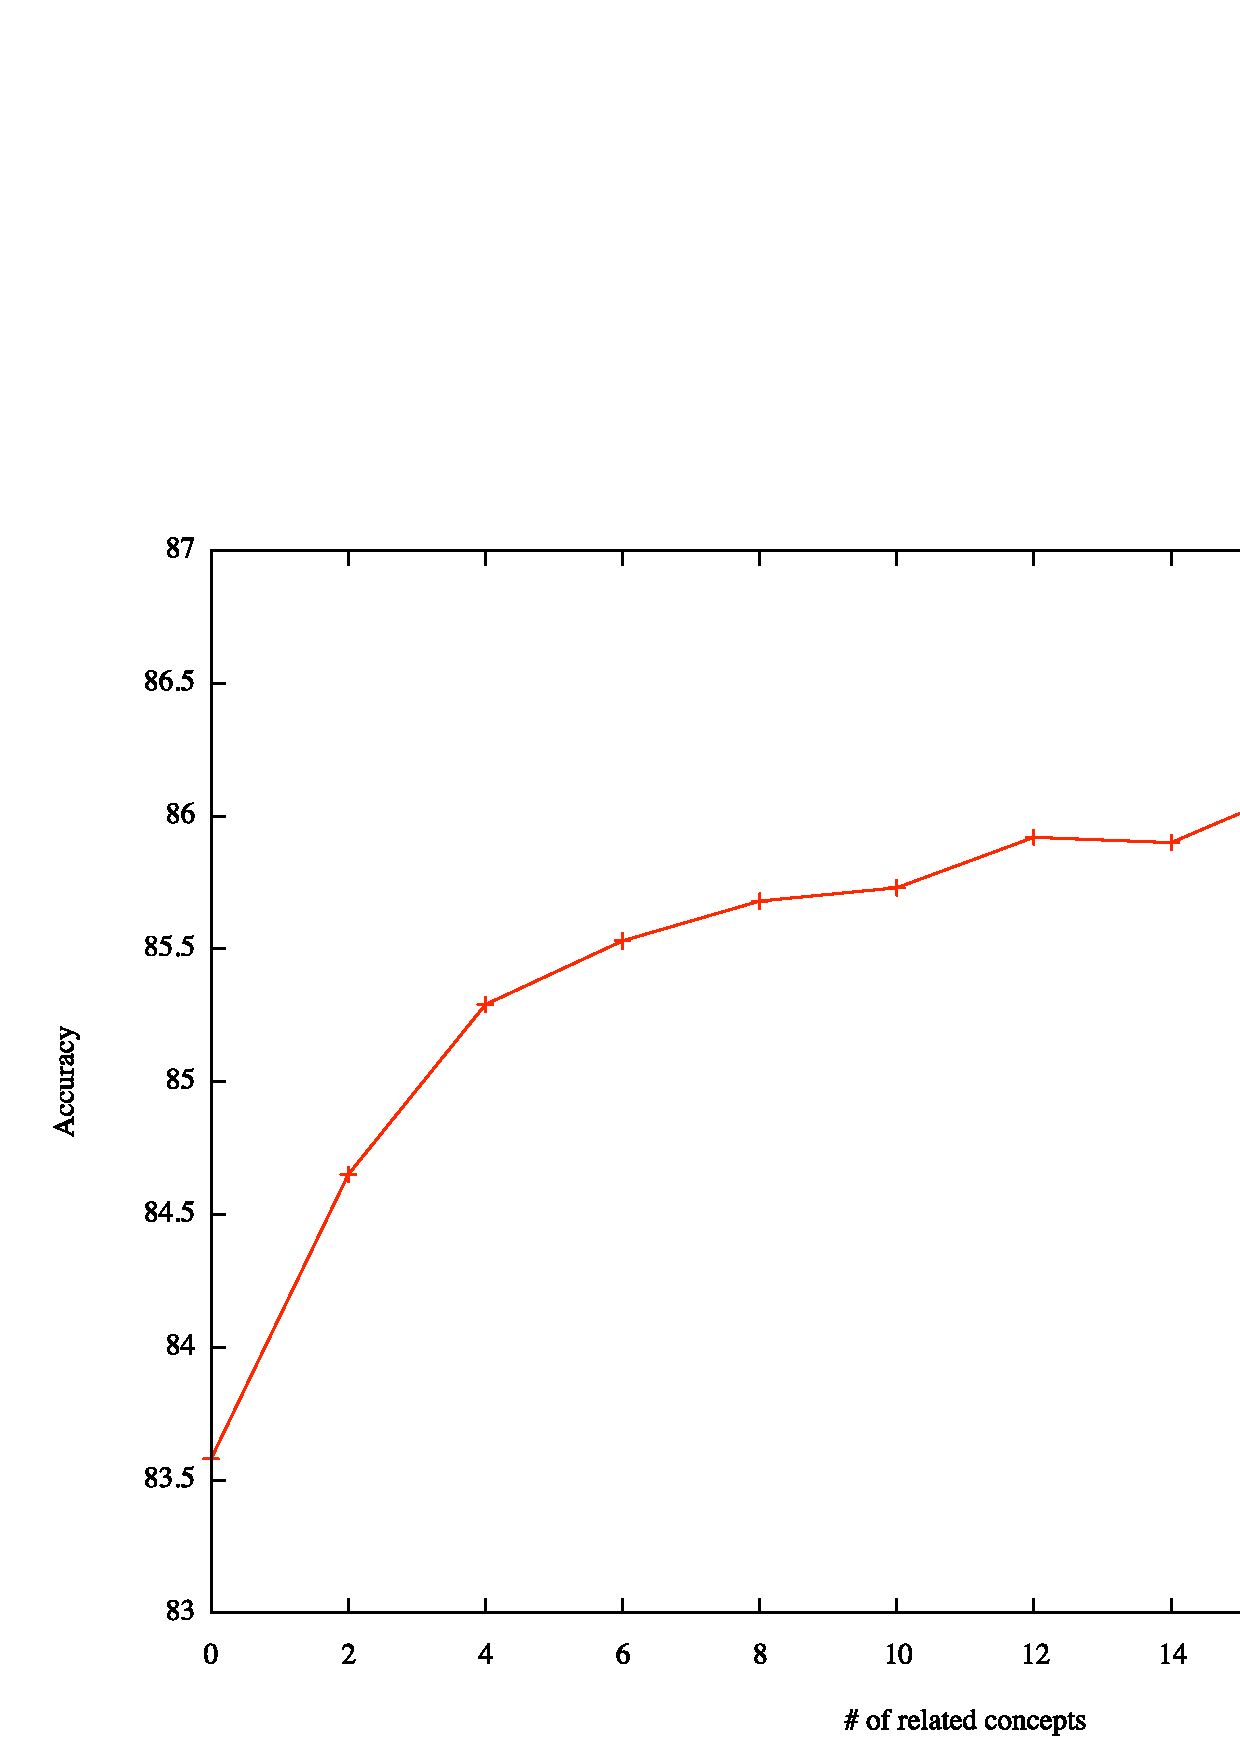
\includegraphics[totalheight=0.25\textheight]{relatedconcepts}
\caption{Relation between system's performance and number of related concepts used in the constraint-based inference model. This experiment is done with the best model of {\em +Inference (Gold)} on the {\em TestAll} test set.}
\label{fig:related-concepts}
\end{figure}

From the graph we see that the improvement keeps increasing when more
related concepts are used. Due to the time limitations, we stop at $22$
related concepts. However, one can expect to obtain better performance
if more related concepts are used.

\ignore{
\subsubsection{Relation Classification Analysis}

In the next experiment, we analyze the performance of our approach on
individual semantic class with $K=3$. We use the {\em TestWiki} test
set as default, except explicitly specified.

\vspace*{2 mm}

{\bf Performance on Individual Semantic Class:} We first analyze our
classifier by looking at the performance on individual semantic
class. This experiment shows us classes which may cause problems to
our classifier. Moreover, this experiment also shows us the
performance of our classifier on individual relation type including $X
\leftarrow Y$, $X \rightarrow Y$, $X \leftrightarrow Y$, and $X
\nleftrightarrow Y$. There are 40 semantic classes in the
datasets. Recall that examples in our datasets are pairs of
concepts. To get the total number of pairs of a semantic class, we
count the number of examples having one of the two concepts belongs to
that class. If two concepts of a pair hold a sibling relation
(i.e. they are in the same semantic class), the pair is counted only
one time for the class. Again, the performance of the classifier is
measured in accuracy which is the portion of correct prediction over
the total number of examples. Table \ref{tab:exp-ind-class} presents
the performance of our classifier on individual semantic class, and
also the average accuracy on each relation type.

From the last row in the table, the average accuracies of the
classifier on relations $X \leftarrow Y$ and $X \rightarrow Y$ are
roughly the same. This essentially occurs because these two learning
classes are symmetric. The performance of the classifier on sibling
relation is lower than other relations. This can be explained by the
fact that disambiguating two sibling concepts is not a trivial
problem. As we discussed in the experiment evaluating the concept
disambiguation algorithm above, two sibling concepts such as two
rivers are not often mentioned in the same article. This fact may
cause the algorithm to retrieve unexpected articles that associate
with two input concepts. This leads to making wrong classification
decision. The ancestor relation, in both directions, gets the best
performance. One of the reason for this result is that disambiguating
two concept holding true ancestor relation is often easy because the
ancestor concept automatically disambiguate the descendant concept in
the pair.

% \textcolor{red}{What should be other discussion on this big table?}
\begin{table}[h]
\tiny
\begin{center}
  \begin{tabular}{|l||c|c|c|c||c|}
    \hline
    \textbf{Semantic class}    & \textbf{$X \leftarrow Y$} & \textbf{$X \rightarrow Y$} & \textbf{$X \leftrightarrow Y$} & \textbf{$X \nleftrightarrow Y$} & \textbf{Average} \\
    \hline
    \hline
    hurricane         &    100  &    100  &    100  &  97.20  &  \textbf{99.30} \\
    cellphonemodel    &    100  &    100  &    100  &  96.85  &  \textbf{99.21} \\
    carmodel          &    100  &    100  &    100  &  94.12  &  \textbf{98.53} \\
\ignore{    searchengine      &    100  &    100  &    100  &  93.18  &  \textbf{98.30} \\
    nationalpark      &    100  &    100  &    100  &  90.51  &  \textbf{97.63} \\
    aircraftmodel     &    100  &    100  &  95.65  &  94.32  &  \textbf{97.49} \\
    nbateam           &    100  &    100  &    100  &  87.88  &  \textbf{96.97} \\
    videogame         &  98.43  &  99.31  &    100  &  87.59  &  \textbf{96.33} \\
    skyscraper        &    100  &    100  &  93.85  &  90.55  &  \textbf{96.10} \\
    digitalcamera     &  91.89  &  94.87  &    100  &  92.96  &  \textbf{94.93} \\
    stadium           &    100  &    100  &  93.59  &  85.06  &  \textbf{94.66} \\
    soccerclub        &    100  &    100  &  97.14  &  80.71  &  \textbf{94.46} \\
    chemicalelem      &    100  &    100  &  90.48  &  86.11  &  \textbf{94.13} \\
    cartooncharacter  &    100  &    100  &  95.83  &  80.30  &  \textbf{94.03} \\
    worldwarbattle    &    100  &    100  &  85.07  &  88.71  &  \textbf{93.45} \\
    treaty            &  93.55  &  94.55  &  89.47  &  92.00  &  \textbf{92.39} \\
    mountain          &    100  &  98.51  &  83.87  &  86.52  &  \textbf{92.23} \\
    university        &    100  &    100  &  83.87  &  82.96  &  \textbf{91.71} \\
    painter           &  97.13  &  96.88  &  77.94  &  93.89  &  \textbf{91.46} \\
    holiday           &  95.45  &    100  &  81.63  &  82.84  &  \textbf{89.98} \\
    newspaper         &  92.13  &  96.88  &  73.44  &  96.64  &  \textbf{89.77} \\
    actor             &  92.74  &  92.24  &  89.47  &  83.33  &  \textbf{89.45} \\
    skybody           &  93.75  &  93.10  &  76.00  &  93.84  &  \textbf{89.17} \\
    wine              &    100  &  86.67  &  80.77  &  86.44  &  \textbf{88.47} \\
    terroristgroup    &    100  &    100  &  68.18  &  83.33  &  \textbf{87.88} \\
    disease           &  85.00  &  87.67  &  81.43  &  95.04  &  \textbf{87.29} \\
    currency          &    100  &  90.00  &  70.00  &  89.06  &  \textbf{87.27} \\
    proglanguage      &  96.55  &  86.67  &  73.44  &  90.97  &  \textbf{86.91} \\
    movie             &  90.23  &  87.06  &  93.62  &  75.91  &  \textbf{86.71} \\
    country           &  98.25  &  98.36  &  91.57  &  57.75  &  \textbf{86.48} \\
    sportevent        &    100  &    100  &  53.19  &  84.00  &  \textbf{84.30} \\
    religion          &  93.88  &  88.57  &  65.88  &  86.40  &  \textbf{83.68} \\
    award             &  96.00  &  98.00  &  41.03  &  92.17  &  \textbf{81.80} \\
    city              &  97.08  &  98.76  &  62.63  &  61.43  &  \textbf{79.98} \\
    flower            &  89.47  &  85.00  &  60.71  &  84.13  &  \textbf{79.83} \\
    basicfood         &  81.82  &  91.11  &  58.89  &  86.11  &  \textbf{79.48} \\
    company           &  93.05  &  94.74  &  55.56  &  74.45  &  \textbf{79.45} \\
    river             &  89.47  &  97.50  &  41.05  &  81.29  &  \textbf{77.33} \\
    drug              &  80.00  &  81.91  &  53.85  &  93.29  &  \textbf{77.26} \\
    empire            &  83.33  &  75.00  &  56.00  &  83.21  &  \textbf{74.39} \\ }
    \hline
    \hline
    \textbf{Average}  & \textbf{95.73}  & \textbf{95.33} & \textbf{80.38} & \textbf{86.58} & \\ %\textbf{0.895}  \\
    \hline
\end{tabular}
\end{center}
\caption{Performance of our system on individual semantic classes.
  The semantic classes are presented in decreasing order of the 
  average accuracy on all relations of the corresponding semantic class. 
  The last row shows the average accuracy of each relation type evaluated on all semantic classes.
  This experiment is done with $K=3$.}
\label{tab:exp-ind-class}
\end{table}


\vspace*{2 mm}

{\bf Internal and External evaluation:} In section
\ref{sec:super-approach}, we argue that our features do not depend on
the semantic class.  We want our classifier to be trained on some
semantic classes and then can be used to identify relations between
concepts in other semantic classes. For example, we do not have
examples in the semantic class {\em fish} in our training data, but we
want to get high accuracy on examples in the class {\em fish} with our
trained classifier. Our features are designed with this as
motivation. In this experiment, we exhibit that our system can indeed
generalize across semantic classes. We present the performance of our
system when trained on some semantic classes and tested on other
classes. We do this experiment using 5-fold cross validation. For each
fold in this experiment, we randomly divide the 40 semantics classes
into two sets. One set gets examples from 30 semantic classes. All
examples in this set are randomly divided into two sub-sets which are
used as the training set and the {\em Internal} test set. The other
set get examples from the other 10 semantic classes and is used as the
{\em External} test set. The results of the 5-fold cross validation
process are showed in table \ref{tab:exp-inter-exter}. We report the
average accuracy of our classifier, which is trained on the training
set in this experiment, applied on both {\em Internal} and {\em
  External} test sets. We learn from the table that our system
performs no worse on the external test set. It is even slightly better
than the performance of the system when applied on the internal test
set. It worth noting that the performance of our system depends on two
important factors: the performance of the concept disambiguation
algorithm and the performance of the relation classifier. If the
classifier is trained on examples from hard semantic classes, such as
the classes at the bottom of table \ref{tab:exp-ind-class}, it may
still perform poorly on the {\em Internal} test set compared to when
it applies on examples in ``easy'' semantic classes, such as classes
at the top of table \ref{tab:exp-ind-class}. This explains why
sometime we may get slightly better results on the {\em External} test
set. The experimental results show that our system generalizes well to
new semantic classes.

\begin{table}[h]
\begin{center}
\begin{tabular}{|c|c|}
\hline
\multicolumn{2}{|c|}{5-fold cross validation} \\
\hline
\hline
Internal Testset & External Testset \\
\hline
88.77 & 89.87 \\
\hline
\end{tabular}
\end{center}
\caption{Genearlization to new classes: Performance of our system on Internal and External test sets using
  5-fold cross validation. The Internal test set is formed by examples having concepts in the same semantic classes as
  those in the train set. The External test set is formed by
  examples having concepts in different semantic classes than those of the train set.
  As shown in this table, this has no significant impact on the results. This experiment is done with $K=3$.}
\label{tab:exp-inter-exter}
\end{table}

\vspace*{2 mm}

{\bf Different sizes of train set:} In this experiment, we present the
performance of our system when the classifier is trained with
different number of examples in the train set. The learning curve of
the average performance is shown in figure
\ref{fig:diff-train-size}. The results show that our system achieves
over 80\% of accuracy by using only 100 examples to train the
classifier. Furthermore, the average performance converges to about
and over 88\% starting with 1,000 examples used in training. The
results illustrate the effectiveness of our system on the problem of
relational knowledge identification.

\begin{figure}[htp]
\centering
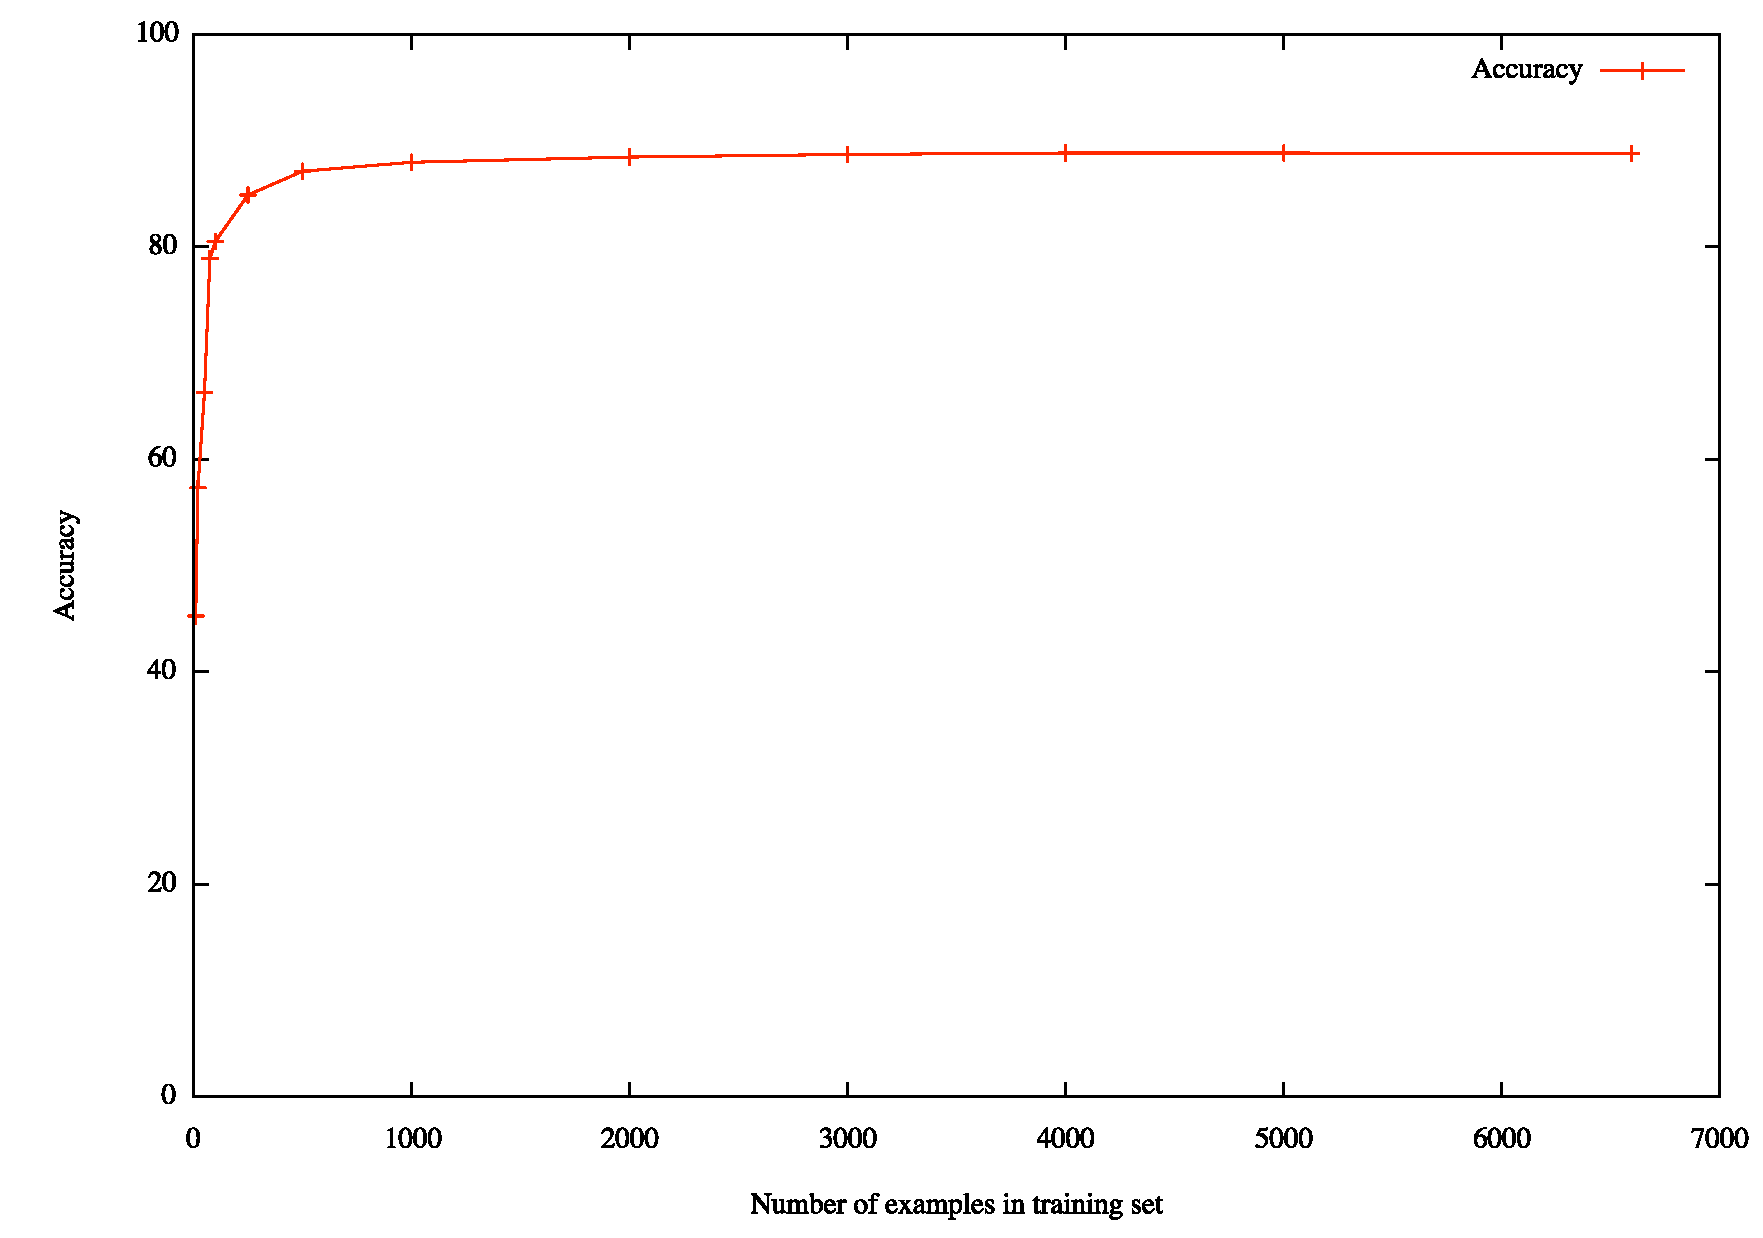
\includegraphics[totalheight=0.25\textheight]{DiffTrainSizes}
\caption{Learning curve of the average performance of our system, as a
  function of the number of training examples. This experiment is done
  with $K=3$ on the {\em TestWiki} test set.}
\label{fig:diff-train-size}
\end{figure}
}

%%% Local Variables: 
%%% mode: latex
%%% TeX-master: "jupiter"
%%% End: 
